\subsection{Spontane Emissions}
	Ein genaues Verständnis dieses Phänomens erfordert eine Quantentheorie des elektromagnetischen Feldes, die man Quantenelektrodynamik (QED) nennt. 
	\\
		
	Betrachte Kasten des Volumens $V = L^3$ \\	
	(Nebenbemerkung: Bei $L \rightarrow \infty$ gibt es infratrot ``Probleme'')
		\begin{align*}
			\vec{A} (\vec{r} , t) &= \vec{\epsilon}~ e^{i (\vec{k} \vec{r} - \omega_k t)} 
			,& \omega_k &= |\vec{k}| \cdot c 
		\end{align*}
	2 orthogonale Polarisationsrichtungen: 
		\begin{align*}
			\vec{\epsilon}_+ \cdot \vec{\epsilon}_- &= 0 
			,& &\vec{k} \cdot \vec{\epsilon}_\pm = 0 \\
			& & &(\text{transversale Welle~} \vec{\nabla} \vec{A} = 0 )
 		\end{align*}
 		\begin{align*}
	 		\vec{\epsilon}_\lambda ~,~ \lambda &\in \{ - , + \} \\
	 		\vec{A} (\vec{r} + L \vec{e}_x , t) &= \vec{A} (\vec{r} , t) &
	 		&\text{für periodische (nicht wichtig) Randbedingungen.} \\
	 		\Rightarrow \vec{k} L \vec{e}_x &= k_x L = 2 \pi n_x &
	 		&\left( e^{i \vec{k} \vec{r}} = e^{i \vec{k} (\vec{r} + L \vec{e}_x)} \right) \\
	 		n_x &\in \mathds{Z}. \\
	 		\vec{k} &= \frac{2 \pi}{L} \vec{n} ,& &n_x, n_y, n_z \in \mathds{Z}
 		\end{align*}
 	Allgemeines
	 	\begin{align*}
		 	\vec{A} (\vec{r} , t) = \frac{c}{\sqrt{2 V}}
		 	\sum_{\vec{k}} \sum_{\lambda \in \{+ , - \} }
		 	\vec{\epsilon}_\lambda (\vec{k}) 
		 	\underbrace{q_\lambda}_{\mathclap{\in \mathds{C}}} (\vec{k} , t) 
		 	e^{-i \vec{k} \vec{r}}
	 	\end{align*}
	Wir fordern $\vec{A} \in \mathds{R}^3$.
		\begin{align*}
			\Rightarrow q_\lambda (- \vec{k} , t) &= q^*_\lambda (\vec{k} , t) ,&
			&\vec{\epsilon}_\lambda (-\vec{k}) = \vec{\epsilon}_\lambda (\vec{k}) \\
			\text{Zusätzlich:~} q_\lambda (\vec{0} , t) &= 0 .& 
			&\text{(nur ebene Wellen)}
		\end{align*}
	Wellengleichung: 
		\begin{align*}
			\left(
				\vec{\nabla}^2 - \frac{1}{c^2} \frac{\partial^2}{\partial t^2} 
			\right)
			\vec{A} (\vec{r} , t) &= \overbrace{0}^{\mathclap{\text{im Vakuum}}} \\
			\overset{\text{Koeff.-Vergleich}}{\Rightarrow} 
			\frac{1}{c^2} \ddot{q}_\lambda (\vec{k} , t) + \vec{k}^2 q_\lambda &= 0
		\end{align*}
		\begin{align*}
			\boxed{\ddot{q}_\lambda (\vec{k} , t) + \omega_k^2 ~q_\lambda (\vec{k} , t)} = 0
		\end{align*}
	$q_\lambda$: Lösungen des harmonischen Oszillators mit Frequenz $\omega_k$. \\
	Energie des elektromagnetischen Feldes: 
		\begin{align*}
			E &= \int_V \diff^3 r ~u (\vec{r} , t) \\
			&= \int_V \diff^3 r \frac{1}{2} \left( \vec{E}^2 (\vec{r} , t) \vec{B}^2 (\vec{r} , t)
			\right) \\
			&= \frac{1}{2} \int_V \diff^3 r \left[
				\left(\frac{1}{c^2} \frac{\partial \vec{A}}{\partial t}\right)^2
				+ \left( \vec{\nabla} \times \vec{A}\right)^2
			\right] \\
			\left( \vec{\nabla} \times \vec{A}\right)^2 &=
			\vec{\nabla} \left(\vec{A} \times \left( \vec{\nabla} \times \vec{A} \right)\right)
			+ \left(\vec{A} \cdot \vec{\nabla}\right) 
			\underbrace{\left( \vec{\nabla} \cdot \vec{A}\right)}_{\mathclap{=0 \text{~(Coulombeichung)}}}
			- \vec{A} \cdot \vec{\nabla}^2 \cdot \vec{A} \\
			\text{zu der Klammer~} &\text{mit mehreren Rotationen:~} \\
			\int_V \diff^3 r~ \vec{\nabla} (\ldots) 
			&= \int_{\partial V} \diff^2 r~ \vec{n} (\vec{r}) (\ldots) = 0
		\end{align*}
		\begin{align*}
			\boxed{
				E = \frac{1}{2} \int \diff^3 r \left[ 
				\left(\frac{1}{c} \frac{\partial \vec{A}}{\partial t}\right)^2
				- \vec{A}~ \vec{\nabla}^2 \vec{A}
				\right]	
			}
		\end{align*}
	Nebenrechnung:
		\begin{align*}
			\int \diff^3 r (\dot{\vec{A}})^2 &= 
			\frac{c^2}{2 V} \sum_{\vec{k}, \lambda} \sum_{\vec{k}', \lambda'}
			\underbrace{\int \diff^3 r e^{i (\vec{k} + \vec{k}') \vec{r}}}_{
				\substack{V \delta_{\vec{k}, -\vec{k}} 
					\text{~für diskretes~} \vec{k},\\ 
					(2 \pi)^3 \delta^{(3)} (\vec{k} + \vec{k}') \\ 
					\text{~kontinuierliches~} \vec{k}}
				}
			\vec{\epsilon}_\lambda(\vec{k}) ~\vec{\epsilon}_{\lambda'} (\vec{k}')
			~\dot{q}_\lambda (\vec{k} , t) ~\dot{q}_{\lambda'} (\vec{k}' , t) 
			\\
			&\overset{\vec{k}' = -\vec{k}'}{=} 
			\frac{c^2}{2} \sum_{\vec{k}, \lambda, \lambda'}
			\vec{\epsilon}_\lambda (\vec{k}) ~\vec{\epsilon}_{\lambda'}(-\vec{k})~
			\dot{q}_\lambda (\vec{k} , t) ~\dot{q}_{\lambda'} (\vec{-k} , t)
			\\
			&= \frac{c^2}{2} \sum_{\vec{k}, \lambda, \lambda'}
			\vec{\epsilon}_\lambda (\vec{k}) ~\vec{\epsilon}_{\lambda'}(-\vec{k})~
			\dot{q}_\lambda (\vec{k} , t) ~\dot{q}^*_{\lambda'} (\vec{k} , t)
			\\
			&= \frac{c^2}{2} \sum_{\vec{k}} \sum_{\lambda \in \{+ , - \} }
			| \dot{q}_\lambda(\vec{k} , t)  |^2
		\end{align*}
	Analog:
		\begin{align*}
			\int_V \diff^3 r \left(- \vec{A} \vec{\nabla}^2 \vec{A}\right)
			&\overset{\text{part. Int.}}{=} \int_V \diff^3 r \left( \vec{\nabla} \vec{A} \right)^2 \\
			&= \frac{c^2}{2} \sum_{\vec{k}} \sum_{\lambda \in \{+ , - \} }
			\vec{k}^2 |q_\lambda (\vec{k} , t)|^2 \\
			E &= \frac{1}{4} \sum_{\vec{k} , \lambda} \left[
				|\dot{q}_\lambda (\vec{k} , t)|^2 + \omega^2_k |q_\lambda (\vec{k} , t)|^2
			\right] \\
			\text{wobei~} |\dot{q}_\lambda (\vec{k} , t)|^2 &= 
			\dot{q}_{1 \lambda}^2 (\vec{k} , t) + \dot{q}_{2 \lambda}^2 (\vec{k} , t) 
			\\
			\text{und~} 
			q_\lambda (\vec{k} , t) &= q_{1 \lambda} (\vec{k} , t) + i q_{2 \lambda} (\vec{k} , t) 
			,& q_{i \lambda} (\vec{k} , t) &\in \mathds{R} 
			\\
			q_\lambda (-\vec{k} , t) &= q_\lambda^* (\vec{k} , t) 
			&\Rightarrow q_{1 \lambda} (-\vec{k} , t) &= q_{1 \lambda} (\vec{k} , t) 
			\\
			& & q_{2 \lambda} (-\vec{k} , t) &= - q_{2 \lambda} (\vec{k} , t)			
		\end{align*}
		\begin{align*}
			E = \frac{1}{2} \sum_{\vec{k} \in H, \lambda}
			\left[
				\dot{q}_{1 \lambda}^2 (\vec{k} , t)
				+ \omega_k^2 ~q_{1 \lambda}^2 (\vec{k} , t)
				+ \dot{q}_{2 \lambda}^2 (\vec{k} , t)
				+ \omega_k^2 ~q_{2 \lambda}^2 (\vec{k} , t)
			\right]
		\end{align*}
	$\vec{k} \in H$ bedeutet $\vec{k}$ ist im Halbraum. z.B. $k_z > 0$
		\begin{align*}
			\text{für~} k_z &= 0 : k_y > 0 \\
			\text{für~} k_z &= k_y = 0 : k_x > 0 
		\end{align*}
	Zu jedem Wellenvektor $\vec{k} \in$ Halbraum und Polarisation $\lambda$ gehören je 2 harmonische Oszillatoren.	
		\begin{align*}
			H_{\text{harm.Oszil.}} &= 
			\frac{p^2}{2 m} + \frac{1}{2} m \omega^2 q^2 \\
			&= \frac{p^2}{2} + \frac{\omega^2}{2} q^2 
			&\text{für~} m &= 1 \text{~ist~} p = \dot{q} \\
			p_{i \lambda} (\vec{k}) \coloneqq \dot{q}_{i \lambda} \\
 		\end{align*}
 	für festes t gilt dann: 
	 	\begin{align*}
	 		H = \frac{1}{2} \sum_{\vec{k} \in H, \lambda}
	 		\left[
		 		p_{1 \lambda}^2 (\vec{k})
		 		+ \omega_k^2 ~q_{1 \lambda}^2 (\vec{k})
		 		+ p_{2 \lambda}^2 (\vec{k})
		 		+ \omega_k^2 ~q_{2 \lambda}^2 (\vec{k})
	 		\right]
	 	\end{align*}
	``quantisiere'' $H$ : $p \mapsto \hat{p} , q \mapsto \hat{q}$
		\begin{align*}
			\left.
			\begin{aligned}
			\left[ \hat{p}_{i \lambda} (\vec{k}) , \hat{q}_{j \lambda'} (\vec{k}')
			\right]
			&= -i\hbar \delta_{ij} \delta_{\lambda \lambda'} \delta_{\vec{k} \vec{k}'} \mathds{1}
			\\
			a_{i \lambda}(\vec{k}) 
			&= \sqrt{\frac{\omega_k}{2 \hbar}} 
			\left(\hat{q}_{i \lambda} (\vec{k}) + \frac{i}{\omega_k} \hat{p}_{i \lambda} (\vec{k})\right)
			\\
			a^\dagger_{i \lambda}(\vec{k})
			&= \sqrt{\frac{\omega_k}{2 \hbar}}
			\left(\hat{q}_{i \lambda} (\vec{k}) - \frac{i}{\omega_k} \hat{p}_{i \lambda} (\vec{k})\right)
			\end{aligned}
			\right\}
			\left[ a_{i \lambda} (\vec{k}) , a_{j \lambda'}^\dagger (\vec{k}')
			\right] 
			= \delta_{ij} \delta_{\lambda \lambda'} \delta_{\vec{k} \vec{k}'} \mathds{1}
		\end{align*}
		\begin{align*}
			\left.
			\begin{aligned}
				a_\lambda (\vec{k}) 
				&\coloneqq \frac{1}{\sqrt{2}} 
				\left(a_{1 \lambda} (\vec{k}) + i a_{2 \lambda} (\vec{k}) \right) \\
				a_\lambda (-\vec{k}) 
				&\coloneqq \frac{1}{\sqrt{2}} 
				\left(a_{1 \lambda} (\vec{k}) - i a_{2 \lambda} (\vec{k}) \right)
			\end{aligned}
			\right\}
			\Rightarrow 
			\begin{aligned}
				&a_\lambda (\vec{k}) \text{~für alle~} \vec{k} \\
				&\vec{k} \in H ~,~ -\vec{k} \in H
			\end{aligned}
		\end{align*}
	Rechnung:
		\begin{equation*}
			\left[
				a_\lambda (\vec{k}), a_{\lambda'}^\dagger (\vec{k}')
			\right]
			= \delta_{\lambda \lambda'} \delta_{\vec{k} \vec{k}'} \mathds{1}
		\end{equation*}
	Einsetzen (Rechnung)
		\begin{align*}
			\vec{A} (\vec{r}) &= 
			\sqrt{\frac{\hbar c^2}{2 V}} \sum_{\vec{k}, \lambda} \frac{1}{\sqrt{\omega_k}}
			\vec{\epsilon}_\lambda (\vec{k}) 
			\left\{ a_\lambda (\vec{k}) e^{i \vec{k} \vec{r}} 
			+ a^\dagger_\lambda (\vec{k}) e^{-i \vec{k} \vec{r}} 
			\right\}
			\\
			H &= 
			\sum_{\vec{k} , \lambda} \hbar \omega_k
			\left( a^\dagger_\lambda (\vec{k}) ~a_\lambda (\vec{k}) + \frac{1}{2}
			\right) & &\text{Problem?}
		\end{align*}
	Energien sind nur bis auf additive Konstante festgelegt. \\
	$E \mapsto E-E_0 ~,~ H \mapsto H - H_0 :$ Term $\frac{\hbar \omega_k}{2}$ hebt sich weg.
	
	Subtraktion der Nullpunktsenergie:
		\begin{align*}
			\boxed{ 
				H \coloneqq 
				\sum_{\vec{k}, \lambda} \left( a^\dagger_\lambda (\vec{k}) ~a_\lambda (\vec{k})\right)
				\hbar \omega_k
			}
		\end{align*}
		\begin{align*}
			H \ket{0} &= \ket{0} ,& 
			H\ket{\vec{k}, \lambda} &= 
			\hbar \omega_k \ket{\overbrace{\vec{k}}^{\mathclap{\text{Photon/Lichtquant}}} , \lambda}
		\end{align*}
	Poyntingvektor
		\begin{equation*}
			\vec{S} = c \vec{E} \times \vec{B}
		\end{equation*}
	Impuls
		\begin{align*}
			\vec{p} &= \int \diff^3 r \underbrace{\vec{S}}_{\mathclap{\text{Impulsdichte}}} 
			= c \int \diff^3 r 
			\left( - \frac{1}{c} \hat{\dot{\vec{A}}} \times (\vec{\nabla} \times \hat{\vec{A}})
			\right) \\
			&\overset{\text{Rechnung}}{=} 
			\sum_{\vec{k} , \lambda} \hbar \vec{k} ~a^\dagger_\lambda (\vec{k}) ~a_\lambda (\vec{k})
		\end{align*}
		\begin{empheq}[box=\boxed]{align*}
			\vec{p} \ket{\vec{k} , \lambda} = \hbar \vec{k} \ket{\vec{k} , \lambda}
		\end{empheq}
		Beim letzten Mal hatten wir $\vec{A} (\vec{r}, t)$ quantisiert wie folgt:\marginpar{29.10.2015}
		\begin{align*}
		\hat{\vec{A}} (\vec{r})= \sqrt{\frac{\hbar}{2V}} ~c
		\sum_{\vec{k}, \lambda \in \{+ , i\}}
		\frac{1}{\sqrt{\omega_k}} \vec{\epsilon}_\lambda (\vec{k}) 
		\left\{ a_\lambda (\vec{k}) e^{i \vec{k} \vec{r}}
		+ a^\dagger_\lambda (\vec{k}) e^{-i \vec{k} \vec{r}}
		\right\}
		\end{align*}
		Wobei
		\begin{align*}
		a^\dagger_\lambda (\vec{k}) \ket{0} 
		&= \overbrace{\ket{\lambda, \vec{k}}}^{\mathclap{\text{Photon}}} \\
		a_\lambda (\vec{k}) \ket{0} &= 0 \\
		\vec{\epsilon}_\lambda (\vec{k}) &: \text{Polarisation} \\
		\hat{\vec{A}} (\vec{r}) &: \text{Operator (keine gewöhnliche Welle)} \\
		\hat{\vec{A}} (\vec{r}) \ket{0} &= \vec{A} (\vec{r})\ket{0} 
		\end{align*}
		D.h $\vec{A} (\vec{r})$ ist ein Eigenwert und enthält keine $a$ oder $a^\dagger$.
		\begin{empheq}[box=\boxed]{align*}
		H = \sum_{\vec{k}, \lambda} \hbar \omega_k
		\underbrace{a^\dagger_\lambda (\vec{k})~a_\lambda (\vec{k})}_{\substack{\text{Nummern oder} \\ \text{Teilchenoperator}}}
		\end{empheq}
		Wobei $\omega_k = c |\vec{k}|$ und kein $\frac{1}{2} \hbar \omega$ vorhanden ist, was damit zutun hat, dass wir nur den Grundzustand betrachten (glaube ich \^{}\^{}).
		
		Auf jeden Fall gilt für $n=1$:
		\begin{align*}
		H \ket{\lambda, \vec{k}} &= \hbar \omega_k \ket{\lambda , \vec{k}} \\
		\hat{\vec{p}} &= \hbar \vec{k} \ket{\lambda , \vec{k}} \\
		E = |\vec{p}| c &\curvearrowright H = |\hat{p}| c \\
		H \ket{0} (&= E_0 \ket{0} = 0 \ket{0} ) = 0
		\end{align*}
		Unendliches Volumen: 
		\begin{align*}
		\frac{1}{V} \sum_{\vec{k}} &\longmapsto \int \frac{\diff^3 k}{(2 \pi)^3}
		& \text{Wobei das~} \vec{k} \text{~so aufgebaut ist:~}k_i &= n_i \frac{2 \pi}{L}, n_i \in \mathds{Z}
		\end{align*} \marginpar{Bleibt die Frage, was $n_i$ sind}
		\begin{align*}
		V \delta_{\vec{k} , 0} &\longmapsto (2 \pi)^2 \delta^{(3)} (\vec{k}) \\
		a_\lambda (\vec{k}) &\longmapsto \frac{1}{\sqrt{\lambda}} 
		& &\text{(wegen Infrarot cutoff)}
		\end{align*} \marginpar{kA was das genau ist}
		\begin{align*}
		\vec{A} (\vec{r}) =
		\sqrt{\hbar} \int \frac{\diff^3 k}{(2 \pi)^3} \frac{c}{\sqrt{2 \omega_k}}
		\sum_\lambda \vec{\epsilon}_\lambda (\vec{k})
		\left\{ a_\lambda (\vec{k}) e^{i \vec{k} \vec{r}}
		+ a^\dagger_\lambda (\vec{k}) e^{-i \vec{k} \vec{r}}
		\right\}
		\end{align*}
		Wir betrachten ab jetzt den Fall: 
		\begin{figure*} [ht]
			\begin{center}
				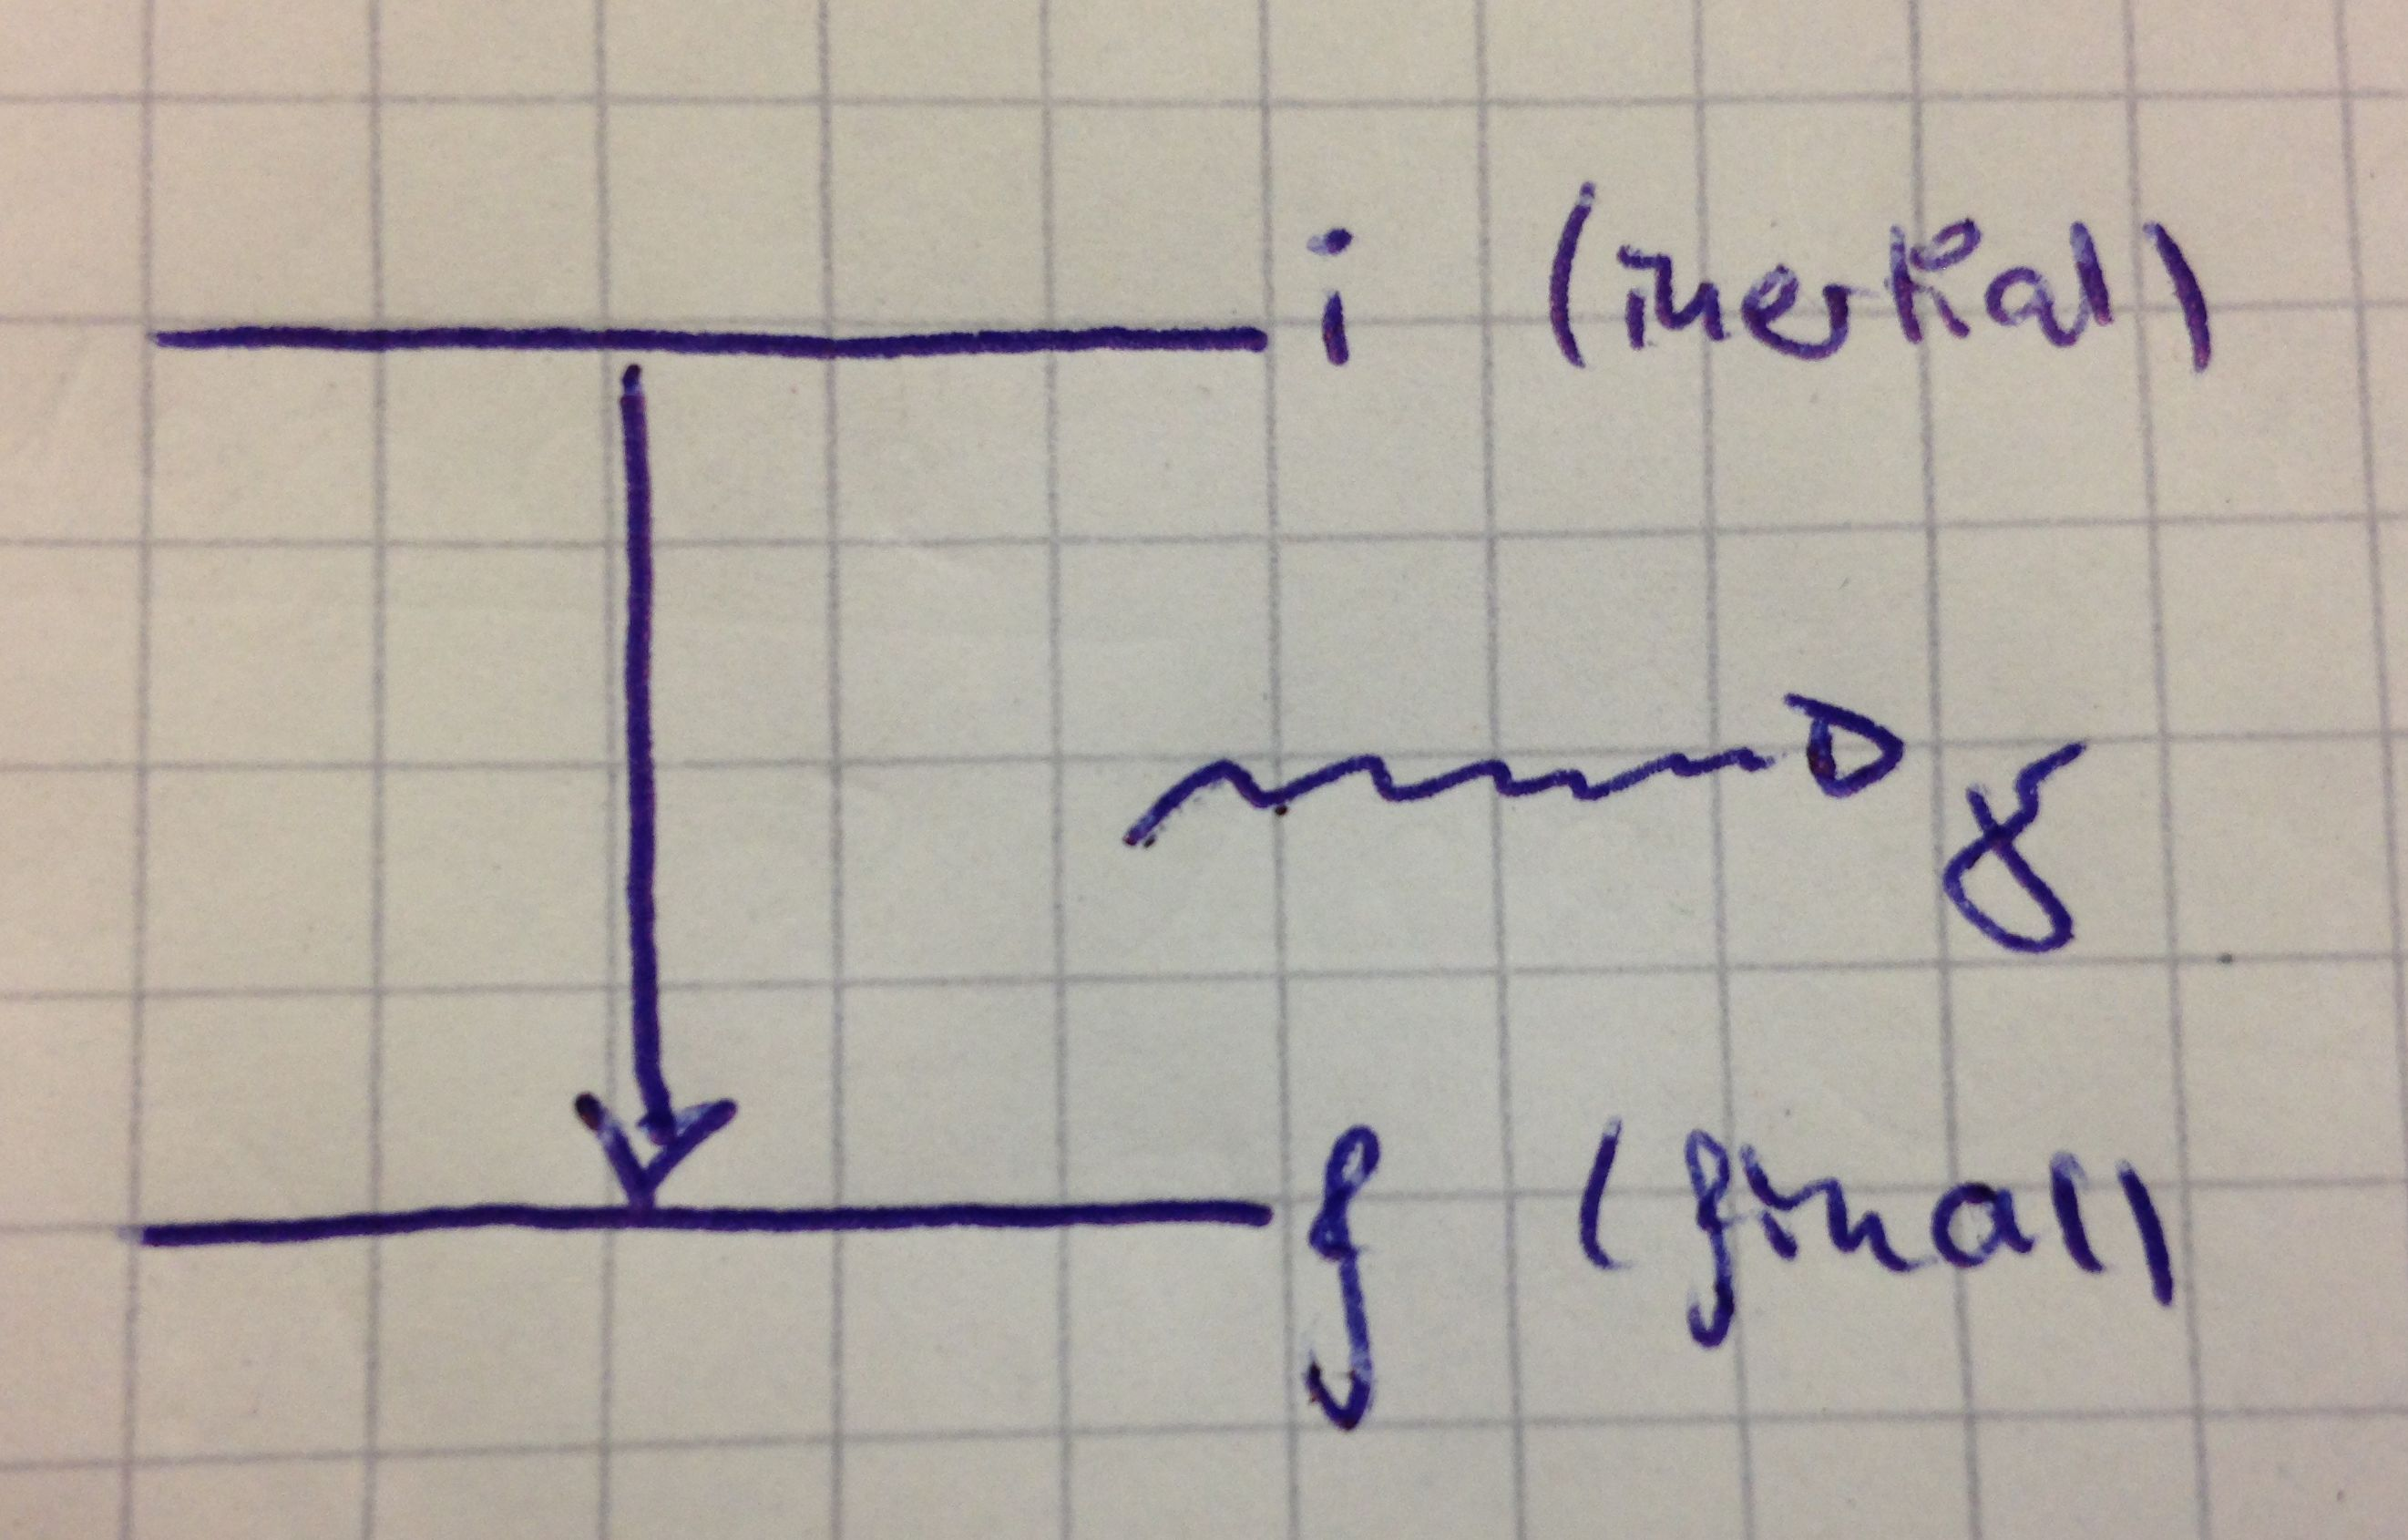
\includegraphics[width=10cm]{Bild2.jpg}
			\end{center}
		\end{figure*}
		\begin{align*}
		H &= H_e + H_\gamma & H_e &: \text{für Elektron}, ~ H_\gamma : \text{für Photon} \\
		H_e &= \underbrace{\frac{\vec{p}^2}{2 m_e} - e \Phi}_{\mathclap{H_e^0}}
		+ \frac{e \vec{A} \vec{p}}{m c}
		+ \frac{e^2}{2 m c^2} \vec{A}^2 &
		&\text{(Coulombeichung)}\\
		&= H_e^0 + H^1 + H^2 \\
		H_e^0 &= \frac{\vec{p}^2}{2 m} - Z \alpha \hbar c \frac{1}{r} & 
		Z &~\text{ist Kernladung},~ \alpha = \frac{e^2}{4 \pi \hbar c}\\
		H_e^0 \ket{n} &= E_n \ket{n} = \hbar \omega_n \ket{n} & 
		\ket{n} &~ \text{ist Elektronzustand}
		\end{align*}	
		für ein H-Atom:
		\begin{align*}
		E_n &= - \frac{1}{2} (Z \alpha)^2 m c^2 \frac{1}{n^2}
		= \frac{1}{2} Z \alpha \hbar c \overbrace{\erw{r^{-1}}}^{\mathclap{\frac{Z}{a_B n^2}}}
		= - \frac{1}{2 n^2} \frac{Z^2 \alpha \hbar c}{a_B} &
		a_B &= \frac{\hbar}{m \alpha c} \\
		H_\gamma &= \int \frac{\diff^3 k}{(2 \pi)^3}
		\sum_{\lambda \in \{+,-\}} \hbar \omega_k
		~a_\lambda (\vec{k})~a^\dagger_\lambda (\vec{k})
		\end{align*}
		Anfangszustand: 
		\begin{align*}
		\ket{i} &= \ket{n(\ell, \ell_z); 0} = \ket{n} \otimes \ket{0}
		\end{align*}
		wobei im \underline{ersten Term} $n$ die Hauptquantenzahl ist, die $\ell$'s sind eigentlich immer da, aber aus Faulheit schreiben wir die fast nie mit, die $0$ bedeutet, dass wir kein Photon haben. Im \underline{zweiten Term} ist $\ket{n}$ der Zustand vom H-Atom und $\ket{0}$ der Zustand von der elektromagnetischen Welle.
		
		Endzustand:
		\begin{align*}
		\ket{f} &= \ket{m(\ell', \ell_z'); \vec{k}, \lambda} 
		= \ket{m} \otimes \ket{\vec{k}, \lambda}
		\end{align*} 
		Der Energieunterschied ist dann:\footnote{Ich habe den Betrag in $\omega_{mn}$ gesetzt, damit wir nicht mit Minuszeichen oder so durcheinander kommen.}
		\begin{align*}
		\Delta E &= E_f - E_i = \hbar 
		\underbrace{(|\omega_m - \omega_n)|}_{\mathclap{\omega_{mn}}} 
		+ \hbar c |\vec{k}| = \hbar (\omega_{mn} + \omega_k)
		\end{align*}
		Übergangsrate: 
		\begin{align*}
		W_{f \leftarrow i} &= 
		\int \frac{\diff^3 k}{(2 \pi)^3} \sum_\lambda
		\frac{2 \pi}{\hbar^2} \delta(\omega_{mn} + \omega_k)
		\left|\braket{f | H_e^1 + H_e^2 | i}\right|^2
		\end{align*}	
		Und $H_e^1 + H_e^2$ ist die Störung (Lösung für $H_e^0 + H_\gamma$ ist bekannt).
		
		Mit Hilfe von
		\begin{align*}
		\int \diff^3 k &= \int \diff k ~k^2 \int \diff \Omega_k
		= \frac{1}{c^3} \int \diff \omega_k ~\omega^2 \int \diff \Omega_k
		\end{align*}
		Können wir schreiben:
		\begin{align*}
		W_{f \leftarrow i} &= \int \diff \Omega_k 
		\frac{\omega_{mn}^2}{4 \pi^2 \hbar^2 c^3}
		\sum_\lambda 
		\left|\braket{f | H_e^1 + H_e^2 | i}\right|^2 \\
		\braket{f | H_e^1 | i} &= 
		\frac{e}{mc} \braket{m | \braket{\vec{k} , \lambda | \hat{\vec{A}}(\vec{k}) | 0} \hat{p} | n} & &\vec{A}\text{~Operator nicht diagonal}\\
		\braket{\vec{k} ,\lambda | \vec{A} (\vec{r}) | 0} &= 
		\sqrt{\hbar} \int \frac{\diff^3 k'}{(2 \pi)^3} \frac{c}{\sqrt{2 \omega_k}}
		\sum_{\lambda'} \vec{\epsilon}_{\lambda'} (\vec{k}') e^{-i \vec{k}' \vec{r}} 
		\cdot \braket{0 | a_\lambda (\vec{k}) a_{\lambda'} (\vec{k}') | 0} 
		& &\text{im Photonraum} 
		\end{align*} 
		Hierbei ist gut zu wissen, dass $\ket{\vec{k} , \lambda} = a_\lambda^\dagger \ket{0}$ und $\bra{\vec{k}, \lambda} = \bra{0}a_\lambda (\vec{k})$.
		\begin{align*}
		\braket{0 | a_\lambda (\vec{k}) a_{\lambda'} (\vec{k}') | 0} &=
		\braket{0 | 
			\underbrace{\left[ a_\lambda (\vec{k}), a_{\lambda'} (\vec{k}') \right]}_{\mathclap{\delta_{\lambda \lambda'} (2 \pi)^3 \delta^{(3)}(\vec{k} - \vec{k'}) \mathds{1}}}  
			| 0} \\
		\braket{\vec{k}, \lambda | \vec{A} (\vec{r}) | 0} &=
		\sqrt{\frac{\hbar}{2 \omega_k}} c~ \vec{\epsilon}_\lambda (\vec{k}) e^{-i \vec{k} \vec{r}} \\
		\braket{f | H_e^1 | i} &= 
		\frac{e}{m} \sqrt{\frac{\hbar}{2 \omega_k}}
		\braket{m | e^{-i \vec{k} \vec{r}} \vec{\epsilon} \vec{p} | n} 
		\end{align*}
		Im Übrigen gilt $\omega_k = |\omega_n - \omega_m| = |-\omega_{mn}| = |\omega_{nm}|$ (siehe $\delta-$Fkt. oben)
		
		Dipolapproximation:
		\begin{align*}
		e^{-i \vec{k} \vec{r}} &= 1 + \mathscr{O} (Z\alpha) \\
		\vec{p} &= \frac{m}{\hbar} i \left[H_e^0, \vec{r}\right] \\
		\Rightarrow 
		\braket{f | H_e^1 | i} &= 
		\frac{-i e}{\sqrt{2}} \sqrt{\hbar \omega_k} 
		\braket{m | \vec{\epsilon}_\lambda \cdot \vec{r}| n}
		\end{align*}
		\begin{align*}
		W_{f \leftarrow i} &= \frac{\omega_{mn}^2 e^2}{8 \pi^2 \hbar c^3}
		\int \diff \Omega_k \sum_\lambda \left|\braket{m | \vec{\epsilon}_\lambda (\vec{k}) ~\vec{r} | n}\right|^2
		\end{align*}
		Der Beitrag im Betrag ins Quadrat ist
		\begin{align*}
		\vec{\epsilon}_{\lambda i}^{~*} (\vec{k}) ~\vec{\epsilon}_{\lambda j} (\vec{k}) 
		\braket{m | r_i | n} \braket{n | r_j | m}
		\end{align*}
		Und mit dem Integral:
		\begin{align*}
		\int \diff \Omega_k (\vec{\epsilon}_{\lambda i}(\vec{k}))^2 &= \frac{4 \pi}{3} \\
		\frac{1}{4 \pi} \int \diff \Omega_k \sum_\lambda 
		\vec{\epsilon}_{\lambda i} (\vec{k}) ~\vec{\epsilon}_{\lambda j} (\vec{k}) 
		&= \frac{2}{3} \delta_{ij}
		\end{align*}
		Somit haben wir nun die Übergangsrate für Spontane Emission in Dipolapproximation:
		\begin{empheq}[box=\boxed]{align*}
		W_{f \leftarrow i} = \frac{\omega^3_{nm} e^2}{3 \pi \hbar c^3}
		\left|\braket{m | \vec{r} | n}\right|^2 
		= \frac{4}{3} \frac{\omega_{nm}^3 \alpha}{c^2}
		\left|\braket{m | \vec{r} | n}\right|^2
		\end{empheq}
		Spontane Emission:
		\begin{equation*}
		W_{m \leftarrow n} = A_{mn} = \frac{4}{3} \frac{\omega_{nm}^3 \alpha}{c^2}
		\left|\braket{m | \vec{r} | n}\right|^2
		\end{equation*}
		Induzierte Emission:
		\begin{equation*}
		W_{m \leftarrow n} = B_{mn} u (\omega_{nm})
		= \frac{4 \pi e^2}{3 \hbar^2} \left|\braket{m | \vec{r} | n}\right|^2
		u (\omega_{nm})
		\end{equation*}
		Induzierte Absorption
		\begin{equation*}
		W_{n \leftarrow m} = B_{nm} u(\omega_{nm})
		\end{equation*}
		Und $B_{mn} = B_{nm}$ sind Einsteinkoeffizienten.
		
		$N_n$ Atome im Zustand $\ket{n}$
		
		$N_m$ Atome im Zustand $\ket{m}$
		
		Leistung:
		\begin{align*}
		&\text{Spontane Emission} & &:  
		&P_{SE} &= 
		\overbrace{N_n A_{mn}}^{\mathclap{\text{Rate~} \left[\frac{1}{\text{Zeit}}\right]}} 
		\underbrace{\hbar \omega_{nm}}_{\mathclap{\text{Energie}}}\\
		&\text{Induzierte Emission} & &:
		&P_{IE} &= N_n B_{mn} ~\hbar \omega_{nm} ~u(\omega_{nm})\\
		&\text{Induzierte Absorption} & &:
		&P_{IA} &= N_m B_{mn} ~\hbar \omega_{mn} ~u(\omega_{nm}) < 0
		\end{align*}
		2 Zustandssysteme $\ket{n}$, $\ket{m}$ im Wärmebad von Photonen im Gleichgewicht: 
		\begin{align*}
		N_n A_{mn} + (N_n B_{mn} - N_m B_{mn}) ~u(\omega_{nm}) &= 0 \\
		N_n &= \gamma \overbrace{e^{- \beta E_n}}^{\mathclap{Boltzmannfaktor}} 
		,& N_m &= \gamma e^{-\beta E_m}
		\end{align*}
		mit $\beta = \frac{1}{k_B ~T}$ \\
		$T$: Temperatur und $\gamma$: Konstante
		\begin{align*}
		\Rightarrow 
		e^{-\beta \hbar \omega_n} \left( A_{mn} + B_{mn} u(\omega_{nm}) \right)
		&= e^{-\beta \hbar \omega_{m}} B_{mn} u(\omega_{nm}) \\
		\Leftrightarrow u(\omega_{nm}) &= \frac{A_{mn}}{B_{mn}} \frac{1}{e^{\beta \hbar \omega_{mn}} - 1}
		\end{align*}
		Und das ist die Energiedichte des elektromagnetischen Feldes im thermischen Gleichgewicht $\left(T=\frac{1}{k_B \beta}\right)$.
		
		Planck:
		\begin{align*}
		\frac{A_{mn}}{B_{mn}} &= \frac{\hbar \omega_{nm}^3}{\pi^2 c^3} \\
		B_{mn} &= \frac{\pi e^2}{3 \hbar^2} \left|\braket{n | \vec{r} | m}\right|^2 \\
		A_{mn} &= \frac{\omega_{mn}^3 e^2}{3 \pi \hbar c^3} \left|\braket{n | \vec{r} | m}\right|^2 
		= \frac{4}{3} \frac{\omega_{mn}^3}{c^2} \alpha \left|\braket{n | \vec{r} | m}\right|^2 
		\end{align*}